%%%%%%%%%%%%%%%%%%%%%%%%%%%%%%%%%%%%%%%%%
% Journal Article
% LaTeX Template
% Version 1.3 (9/9/13)
%
% This template has been downloaded from:
% http://www.LaTeXTemplates.com
%
% Original author:
% Frits Wenneker (http://www.howtotex.com)
%
% License:
% CC BY-NC-SA 3.0 (http://creativecommons.org/licenses/by-nc-sa/3.0/)
%
%%%%%%%%%%%%%%%%%%%%%%%%%%%%%%%%%%%%%%%%%

%----------------------------------------------------------------------------------------
%	PACKAGES AND OTHER DOCUMENT CONFIGURATIONS
%----------------------------------------------------------------------------------------

\documentclass[twoside]{article}
\usepackage{graphicx}

\usepackage[sc]{mathpazo} % Use the Palatino font
\usepackage[T1]{fontenc} % Use 8-bit encoding that has 256 glyphs
\linespread{1.05} % Line spacing - Palatino needs more space between lines
\usepackage{microtype} % Slightly tweak font spacing for aesthetics

\usepackage[hmarginratio=1:1,top=32mm,columnsep=20pt]{geometry} % Document margins
\usepackage{multicol} % Used for the two-column layout of the document
\usepackage[hang, small,labelfont=bf,up,textfont=it,up]{caption} % Custom captions under/above floats in tables or figures
\usepackage{booktabs} % Horizontal rules in tables
\usepackage{float} % Required for tables and figures in the multi-column environment - they need to be placed in specific locations with the [H] (e.g. \begin{table}[H])
\usepackage{hyperref} % For hyperlinks in the PDF

\usepackage{lettrine} % The lettrine is the first enlarged letter at the beginning of the text
\usepackage{paralist} % Used for the compactitem environment which makes bullet points with less space between them

\usepackage{abstract} % Allows abstract customization
\renewcommand{\abstractnamefont}{\normalfont\bfseries} % Set the "Abstract" text to bold
\renewcommand{\abstracttextfont}{\normalfont\small\itshape} % Set the abstract itself to small italic text

\usepackage{titlesec} % Allows customization of titles
\renewcommand\thesection{\Roman{section}} % Roman numerals for the sections
\renewcommand\thesubsection{\arabic{subsection}} % Roman numerals for subsections
\titleformat{\section}[block]{\large\scshape\centering}{\thesection.}{1em}{} % Change the look of the section titles
\titleformat{\subsection}[block]{\large}{\thesubsection.}{1em}{} % Change the look of the section titles

\usepackage{fancyhdr} % Headers and footers
\pagestyle{fancy} % All pages have headers and footers
\fancyhead{} % Blank out the default header
\fancyfoot{} % Blank out the default footer
\fancyhead[C]{PPGEB - FEELT - UFU $\bullet$ 2013/2} % Custom header text
\fancyfoot[RO,LE]{\thepage} % Custom footer text

\usepackage[utf8]{inputenc}
\usepackage{graphicx}
\graphicspath{{imgs/}}

\usepackage{listings}
\usepackage{xcolor}

\lstdefinestyle{sharpc}{language=[Sharp]C, frame=lr, rulecolor=\color{blue!80!black}, breaklines=true}

%----------------------------------------------------------------------------------------
%	TITLE SECTION
%----------------------------------------------------------------------------------------

\title{\vspace{-15mm}\fontsize{24pt}{10pt}\selectfont\textbf{Algoritmo genético para resolução do problema do caixeiro viajante (TSP)}} % Article title

\author{
\large
\textsc{Daniel Teodoro Gonçalves Mariano, Keiji Yamanaka (Ph.D)}\\[2mm] % Your name
\normalsize Universidade Federal de Uberlândia\\ \normalsize Uberlândia-MG, Brasil \\ % Your institution
\normalsize {dtgmariano@gmail.com, keiji@ufu.br} % Your email address
\vspace{-5mm}
}
\date{}

%----------------------------------------------------------------------------------------

\begin{document}

\maketitle % Insert title

\thispagestyle{fancy} % All pages have headers and footers

%----------------------------------------------------------------------------------------
%	ABSTRACT
%----------------------------------------------------------------------------------------


\begin{abstract}
\noindent
Algoritmo genético é uma heurística de busca que simula o processo de evolução das espécies observado em sistemas biológicos. A aplicação vigente consiste no desenvolvimento de um algoritmo genético para encontrar o valor mínimo da função de Schwefel.
\end{abstract}

%----------------------------------------------------------------------------------------
%	ARTICLE CONTENTS
%----------------------------------------------------------------------------------------

\begin{multicols}{2} % Two-column layout throughout the main article text

\section{Introdução}

\subsection{Algoritmos Evolucionários}
Algoritmos evolucionários utilizam modelos computacionais baseados em processos naturais de evolução como um instrumento para a resolução de problemas. Os modelos computacionais propostos se orientam pela simulação de conceitos de evolução das espécies: seleção, mutação e reprodução. Os algoritmos evolucionários operam proporcionando a manutenção de uma população de estruturas, chamadas de indivíduos ou cromossomos. Esses indivíduos se comportam de maneira similar à evolução das espécies, sendo submetidos à operadores genéticos (recombinação e mutação).Cada cromossomo recebe uma avaliação de acordo com o nível de aptidão que este possui dentro do contexto de um problema.

\subsection{Algoritmos Genéticos}
Algoritmos genéticos são um ramo dos algoritmos evolucionários, podendo ser definido como uma técnica de busca baseada numa metáfora do processo biológico de evolução natural. São técnicas heurísticas de otimização global. A otimização global é uma questão que opõe os GAs aos métodos como gradiente (hill climbing), que seguem a derivada de uma função de forma a encontrar o máximo de uma função, ficando facilmente retidos em máximos locais. Nos GAs, populações de indivíduos são criadas e submetidas aos operadores genéticos: seleção, recombinação (crossover) e mutação. Tais operadores utilizam uma caracterização da qualidade de cada individuo como solução do problema em questão chamada de avaliação. Dessa forma geram um processo de evolução natural destes indivíduos, que eventualmente devera gerar um individuo que caracterizara uma boa solução para o nosso problema.

\subsection{Etapas de um AG}
Um AG pode ser dividido nas seguintes etapas:

\begin{enumerate}
\setlength{\itemsep}{0.2cm}%
 \setlength{\parskip}{0.2cm}
\item Inicialização: A população inicial de soluções candidatas são usualmente geradas randomicamente ao longo do espaço de busca. Conhecimentos ou informações específicas do domínio do problema podem ser incorporadas ao algoritmo.
\item Avaliação: Uma vez que a população é iniciada ou uma população descendente é criada, os valores de aptidão das soluções candidatas é avaliada.
\item Seleção: Aloca mais cópias dessas soluções com valores de aptidão superior e, assim, impõe o mecanismo de sobrevivência do mais apto nas soluções candidatas. A idéia principal da seleção é de preferir as melhores soluções em relação as piores.
\item Recombinação: Combina partes de dois ou mais cromossomos (soluções/indivíduos parentais) para gerar um novo cromossomo. Existem diferentes maneiras de se realizar a combinação entre indivíduos. A performance dessa etapa está relacionado com o quão apropriado é o mecanismo de recombinação projetado para aquele contexto. A prole sob recombinação não será idêntico a um pai em particular, pois irá recombinar traços dos pais de uma maneira nova
\item Mutação: Enquanto a recombinação ocorre envolvendo dois ou mais cromossomos a mutação ocorre individualmente. A mutação promove a alteração da solução de maneira randômica. Existem diversas variações de mutações, geralmente envolvendo uma ou mais alterações dos traços de um cromossomo.
\item Reposição: A população criada através da seleção, recombinação e mutação, substituirá os cromossoms pais. 
\item Verificação da condição parada: Enquanto a condição de parada não foi encontrada, repete-se os procedimentos do passo 2 ao 6.
\end{enumerate}

\subsection{Problema do caixeiro viajante (TSP)}
O problema do caixeiro viajante, é um problema de otimização combinatória. Trata-se de uma dada lista de pontos a serem visitados, o problema consiste em encontrar a menor distância a ser percorrida para visitar todos os pontos, sem passar duas vezes pelo mesmo ponto.
O problema pertence à categoria NP-Completo que o remete para um campo de complexidade exponencial, isto é, o esforço computacional necessário para a sua resolução cresce exponencialmente com o tamanho do problema. Assim, dado que é difícil, se não impossível, determinar a solução ótima desta classe de problemas, os métodos de resolução passam pelas heurísticas e afins que, do ponto de vista matemático, não asseguram a obtenção de uma solução ótima.

\begin{figure}[H]
  \caption{Diagrama de blocos de um AG básico.}
  \centering
    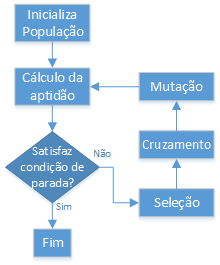
\includegraphics[scale = 1]{basicga_diagram.png}
\end{figure}

%------------------------------------------------

\section{Métodos}
O artigo vigente apresentará a implementação de um algoritmo genético que solucione o problema do caixeiro viajante, utilizando os operadores de cruzamento CX (Cycle Crossover), PMX(Partially Matched Crossover) e o operador de mutação Swap. O software da aplicação foi desenvolvido na plataforma .NET, em linguagem computacional CSharp (C\#).

\subsection{Representação cromossomial}
Para o desenvolvimento do problema é necessário que a informação do problema seja traduzida em uma linguagem apta para o computador manipular. Inicialmente foi gerado o espaço amostral com n cidades dispostas pelo mapa do problema. Cada cidade possui um identificador único e um par de coordenadas (x,y) que representa sua posição no mapa. O cromossomo é composto por uma lista dos identificadores de cada cidade. Um restrição do problema é que um mesmo cromossomo não pode possuir identificadores de uma mesma cidade repetidos ao longo do seu cromossomo. Por esta razão o emprego de métodos de cruzamento tradicionais como o crossover de um ponto, o crossover de dois pontos e o crossover uniforme não são adequadas, uma vez que estes operadores não restrigem a geração de descendentes que tenham informações repetidas no seu cromossomo.
A ordem em que os identificadores das cidades são dispostos pelo cromossomo indicam o trajeto a ser seguido.

\begin{figure}[H]
  \caption{Representação cromossomial para o problema.}
  \centering
    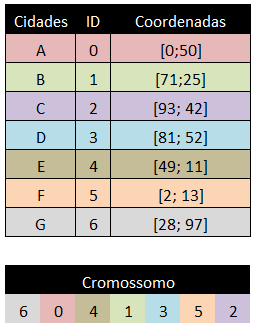
\includegraphics[scale =  0.8]{crom_rep.png}
\end{figure}

Neste exemplo, o caixeiro viajante seguirá o trajeto G -> A -> E -> B -> D -> F -> C.

\subsection{Cálculo de aptidão}
O cálculo de aptidão é a etapa do algoritmo genético em que se determina a qualidade de um indivíduo como soluçao do problema em questão. Cada cromossomo da populaçao é avaliado recendo um valor numérico para representar o seu grau de aptidão. Essa nota servirá de base para a etapa de seleção de pais. Dessa forma os individuos com melhor avaliação terão maior probabilidade de serem escolhidos como pais para a próxima geração de cromossomos. Para o problema tratado nesse artigo, o cálculo de aptidão foi dado pelo inverso do somatório das distâncias entre todas as cidades ao longo do trajeto a ser percorrido pelo caixeiro viajante. 

\begin{equation}
\label{eq:distperc}
distTotal = \sum_{i=0}^{n-1} \sqrt{|x_{i} - x_{i+1}|^2 + |y_{i} - y_{i+1}|^2}
\end{equation}

A função de avaliação é expressa por \ref{eq:fitfunc} :
\begin{equation}
\label{eq:fitfunc}
fit = 1/distTotal
\end{equation}

\subsection{Elitismo}
Trata-se de uma modificação no módulo de população com o intuito de garantir o crescimento positivo do desempenho do AG ao decorrer das gerações. No elitismo os n melhores individuos de cada geração são preservados para a próxima geração.  Em um exemplo de aplicação de elitismo, uma população com 10 cromossomos (AG com elitismo de valor n igual a 2), a cada geração, dois dos melhores indivíduos da população são reservado. Em seguida serão selecionados 8 pais para gerarem 8 descendentes. Os individuos selecionados como elite são adicionados a população após o método de seleção completando os 10 individuos da população.

\subsection{Seleção dos pais}
A etapa de seleçao dos pais é baseado no mecanismo de seleção natural que atua sobre as espécies biológicas. Individuos de uma população que possuem maior aptidão terão maior probabilidade de se tornarem pais e consequentemente gerar descendentes que carreguem parte de sua informaçao genética. Indivíduos menos aptos também podem se tornar pais, embora a probabilidade desse evento ocorrer seja menor. Caso a possibilidade de reproduçao seja restrita apenas aos melhores indivíduos, a populaçao tenderá a ser composta de indivíduos cada vez mais semelhantes e faltará diversidade a esta população para que a evolução possa prosseguir de forma satisfatória. A tal efeito é denominado como convergência genética, podendo ser minimizado ou evitado através da seleçao equilibrada de indivíduos menos aptos da população. Existem diversos métodos de seleção propostos, tais como: seleção por roleta, seleção universal estocástica, seleção por ranking, seleção por torneio, entre outros. Para a aplicação foi utilizado o método de seleção por roleta.

\subsubsection{Método da roleta viciada}
Dada uma população de cromossomos, cada componente é avaliado de forma a determinar o seu nível de aptidão. 
\begin{table}[H]
\caption{Dados de uma dada população}
\centering
\begin{tabular}{cc}
\toprule
Indivíduo & Avaliação \\
\midrule
A & 4\\
B & 1\\
C & 3\\
D & 4\\
E & 5\\
F & 6\\
\bottomrule
\end{tabular}
\end{table}
A probabilidade de seleção de cada indivíduo é determinada de acordo com o seu nível de aptidão em relação ao somatório dos níveis de aptidão de toda a população \ref{eq:ps}. 
\begin{equation}
%\label{eq:p_{s} = probabilidade de seleção}
\label{eq:ps}
ps(i) = \frac {fit(i)}{\sum\limits_{j=1}^n fit(j)} * 100
\end{equation}

Para estabelecer a probabilidade de seleção acumulada dos cromossomos da população é realizada a somatória das probabilidades de seleção do n-ésimo cromosso com a dos cromossomos anteriores conforme demonstrado na equação \ref{eq:psa}.
\begin{equation}
%\label{eq:p_{s} = probabilidade de seleção acumulada}
\label{eq:psa}
psa(i) = \sum\limits_{j=1}^i fit(j)
\end{equation}

A tabela \ref{tab:popinfo} mostra os indivíduos da população com seus valores de avaliação, probabilidade de seleção e probabilidade acumulada de seleção.
\begin{table}[H]
\label{tab:popinfo}
\caption{Distribuiçao das probabilidades (seleção e acumulada)}
\centering
\begin{tabular}{ccll}
\toprule
Indivíduo & Avaliação & Ps (\%) & Psa (\%) \\
\midrule
A & 4 & 17,39 & 17,39\\
B & 1 & 4,35 & 21,74\\
C & 3 & 13,04 & 34,78\\
D & 4 & 17,39 & 52,17\\
E & 5 & 21,74 & 73,91\\
F & 6 & 26,09 & 100,00\\
\bottomrule
\end{tabular}
\end{table}

A partir desses dados é possível visualizar a configuração da roleta conforme a figura \ref{fig:roleta}. Cada individuo é representado por uma fatia da roleta.

\begin{figure}[H]
\label{fig:roleta}
  \caption{Roleta.}
  \centering
    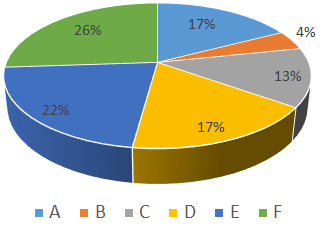
\includegraphics[scale = 0.7]{roleta.png}
\end{figure}

Observa-se que os individuos com maior probabilidade de seleção, ocupam uma área maior da roleta. A probabilidade de seleção de cada indivíduo da população é distribuída em intervalos conforme a figura \ref{fig:ditrib}

\begin{figure}[H]
\label{fig:ditrib}
  \caption{Distribuição.}
  \centering
    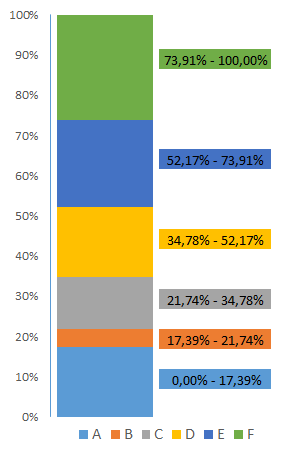
\includegraphics[scale = 0.8]{roleta_dist2.png}
\end{figure}

A partir dessa distribuição, um número randômico dentro do intervalo [0.00\%; 100.00\%] é gerado. Dentro os intervalos de distribuição da roleta, escolhe-se o cromossomo cujo intervalo o número gerado pertencer. O procedimento é repetido n vezes onde n é o tamanho da população.

\subsubsection{Ranking}
A seleção por ranking é um método de seleção que evita a convergência prematura e a dominância de um superindi-víduo. O seu principio consiste em ordenar todos os ele-mentos de acordo com a sua função de avaliação e usar este ranking como base da seleção, ao invés de usar diretamente o valor da avaliação. Uma vez definidos os novos valores de avaliação destes indivíduos, um método tradicional, tal como o da roleta vi-ciada, pode ser utilizado para a escolha dos pais que serão submetidos aos operadores genéticos.


\subsubsection{Torneio}
O método de seleção baseada em um torneio consiste em selecionar uma série de indivíduos da população para competições diretas. Os cromossomos competem diretamente, tendo como critério a função de avaliação de cada um. O cromossomo com melhor avaliação na competição é escolhido como pai. Um parâmetro para o torneio é definir o número de participantes por competição (k).
Em um exemplo de AG tem-se a seguinte população, composta por 8 indivíduos:

\begin{table}[H]
\label{tab:popinfo}
\caption{Exemplo de população}
\centering
\begin{tabular}{cc}
\toprule
Indivíduo & Avaliação\\
\midrule
A & 10\\
B & 5\\
C & 9\\
D & 1\\
E & 3\\
F & 7\\
G & 6\\
H & 2\\
\bottomrule
\end{tabular}
\end{table}

Para um critério k com valor igual a 2, serão selecionados aleatoriamente oito duplas. De cada dupla será reservado o indivíduo com função de avaliação superior.

\begin{figure}[H]
\label{fig:torneio}
  \caption{Exemplo de torneio.}
  \centering
    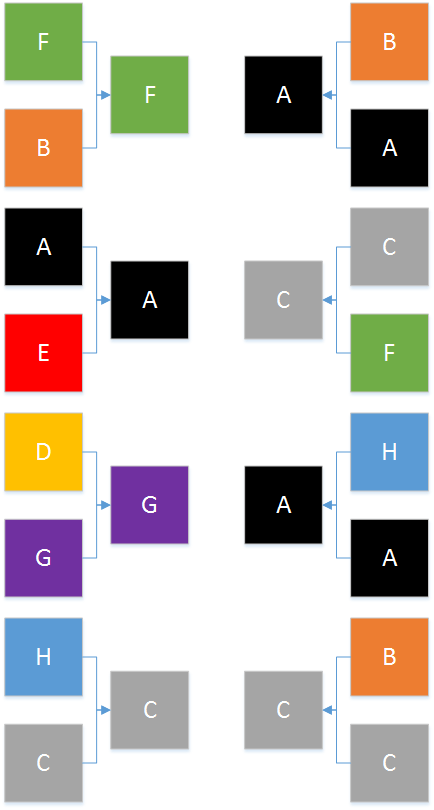
\includegraphics[scale = 0.47]{torneio.png}
\end{figure}

A partir dos indivíduos selecionados por torneio, é que se efetua o processo de cruzamento.

\subsection{Cruzamento (Crossover)}
Crossover é um operador genético usado para reprogramar a configuração de um cromossomo de uma geração para a próxima. Este operador é análogo à reprodução biológica de forma a promover a recombinação genética de duas ou mais soluções progenitoras e consequentemente gerando uma solução descendente. Existem diferentes técnicas de recombinação: com um ponto, com dois pontos,"corta e emenda", uniforme, metade uniforme, com três progenitores, cromossomos ordenados, tendenciosa, entre outras.

\subsubsection{Crossover de um ponto}
Neste cruzmanento, um único ponto para recombinação é selecionado randomicamente para os cromossomos progenitores. Todos os genes a partir deste ponto são trocados entre os cromossomos. Os organismos resultantes são os filhos. A figura \ref{fig:c1p} ilustra um cruzamento de um ponto.

\begin{figure}[H]
\label{fig:c1p}
  \caption{Cruzamento de um ponto.}
  \centering
    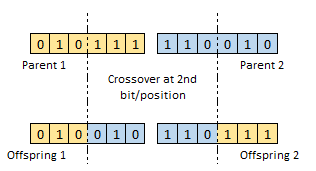
\includegraphics[scale = 0.9]{crossover_onepoint.png}
\end{figure}

Entretanto existe a possibilidade de os pais não realizarem a recombinação. Isto ocorre porque existe uma probabilidade de cruzamento (Pc) a ser considerada inicialmente. Um valor de Pc é definido nas configurações do AG antes do algoritmo ser iniciado. Para cada cromossomo parental é gerado um valor randômico (random) variando entre [0\%; 100\%]. Se a variável random possuir um valor menor ou igual ao valor de Pc, o cruzamento é efetuado. Caso contrário, os individuos não efetuam o cruzemento mantendo suas características para a próxima geração.

\subsubsection{Crossover de dois pontos}
Este cruzamento é semelhante ao cruzamento de um ponto, embora sejam selecionados dois pontos para recombinação. O conteúdo genético delimitado por estes pontos é trocado dos cromossomos progenitores para os cromossomos descendentes. Os demais alelos fora deste intervalo são preservados. A figura \ref{fig:c1p} ilustra o cruzamento de dois pontos.
\begin{figure}[H]
\label{fig:mut}
  \caption{Cruzamento de dois pontos.}
  \centering
    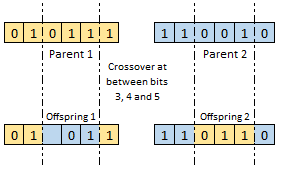
\includegraphics[scale = 0.9]{crossover_twopoints.png}
\end{figure}

\subsubsection{Crossover uniforme}
Para cada gene é sorteado um número 0 ou 1. Se o valor sorteado for igual a 1, o primeiro filho recebe o gene da mesma posição do primeiro pai (de maneira idêntica o segundo filho recebe o gene da mesma posição do segundo pai). Se o valor sorteado for 0, as atribuições serão invertidas: o primeiro filho recebe o gene da posição corrente do segundo pai e o segundo filho recebe o gene corrente do primeiro pai.


\begin{figure}[H]
\label{fig:mut}
  \caption{Cruzamento uniforme.}
  \centering
    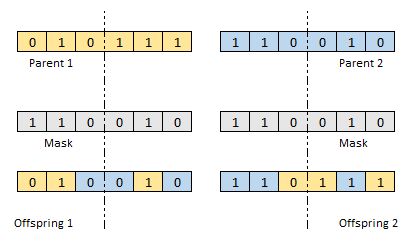
\includegraphics[scale = 0.75]{crossover_uniform.png}
\end{figure}

O crossover uniforme é uma alternativa ao crossover de dois pontos. Enquanto este último possui uma maior probabilidade de seperar partes do cromossomo de grande cromossomo durante o cruzamento, o cruzamento uniforme tende a conservar esquemas longos com a mesma probabilidade que preserva esquemas de menor comprimento, desde que ambos tenham a mesma ordem. Por outro lado, devido ao fato de fazer um sorteio para cada posiçao, este cruzamento tem uma grande possibilidade de estragar todo e qualquer esquema, mas em média o seu desempenho é superior ao cruzamento de um ponto e ao cruzamento de dois pontos.

\subsubsection{Partially Matched Crossover (PMX)}
Sugerido por Goldberg e Lingle , o PMX é um operador de cruzamento que age trocando blocos de genes entre os pais, gerando novos filhos.

\begin{enumerate}
\item Randomicamente seleciona uma porção dos alelos do pai 1 e copia essa mesma porção para o filho 1.Os alelos do filho são organizados de forma que, os alelos que estão fora zona de corte, recebem um valor '*'
\item Procurando no mesmo segmento do Pai 2, seleciona cada valor que ainda não foi copiado para o filho 1.
\item Para cada um desses valores:
\begin{enumerate}
\item Observa o index i desse valor no Pai 2. Localiza-se o valor v que encontra-se nesse no index i no Pai 1. Procura-se o valor v no Pai 2.
\item Se o index desse valor v no Pai 2 fizer parte da porção original, retorne ao passo anterior, utilizando esse valor.
\item Se o index desse valor v no Pai 2 não fizer parte da porção original, insira esse valor no cromossomo do filho 1 na mesma posição.
\end{enumerate}
\item Os valores com '*' no filho 1 recebem os valores de index correspondente do pai 2.
\end{enumerate}

A figura \ref{fig:pmx} ilustra o operador PMX.
\begin{figure}[H]
\label{fig:pmx}
  \caption{PMX}
  \centering
    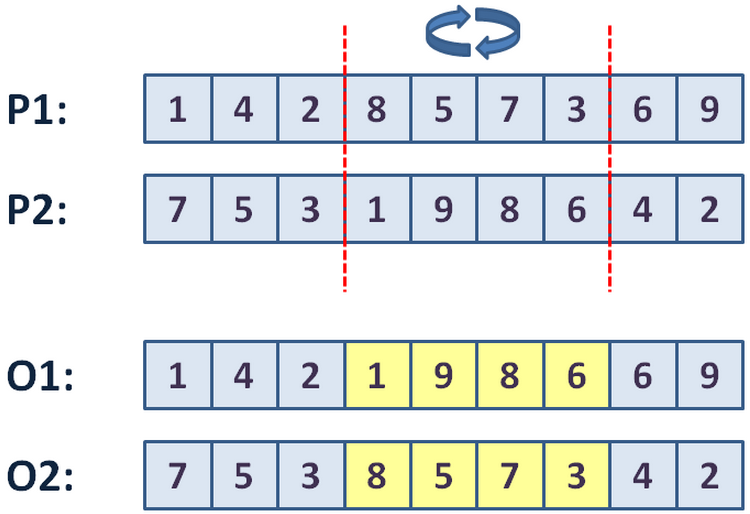
\includegraphics[scale = 0.3]{pmx_crossover.png}
\end{figure}

\subsubsection{Cycle Crossover (CX)}
Proposto por Oliver et al. Este operador gera filhos que preservam a posição absoluta da cidades provenientes dos cromossomos pais. Ele trabalho sobre um subconjunto de cidades que ocupa um mesmo subconjunto de posições em ambos os pais. Estes pontos são copiados de um dos pais, nas mesmas posições, para um filho. As posições remanescentes são completadas com as cidades do outro pai. Assim, cada cidade e sua posição são herdadas de um dos pais. A figura \ref{fig:cx} ilustra o operador CX.
\begin{figure}[H]
\label{fig:cx}
  \caption{CX}
  \centering
    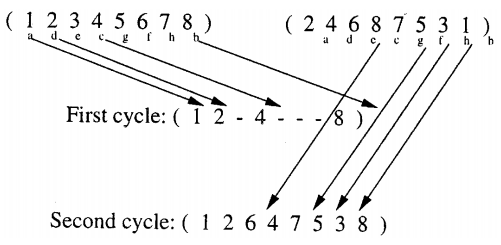
\includegraphics[scale = 0.55]{crossover_cx.png}
\end{figure}

\subsection{Mutação}
A mutação é um operador genético utilizado para manter a diversidade gênica de uma geração de cromossomos para a próxima. É análoga à mutação presente nos sistemas biológicos. Este operador pode alterar um ou mais genes de um cromossomo. De maneira semelhante à etapa de cruzamento, a mutação possui uma probabilidade associada (Pm), que define a chance de tal processo ocorrer em um determinado momento. Um variável randômica, pertencente ao intervalo [0\%; 100\%], é gerada. Se o valor dessa variável for inferior ou igual à Pm, a mutação ocorre. Se for superior, a operação não é realizada e o cromossomo mantém suas características sem alterações. Existem diferentes tipos de mutação: inversão de um único bit, inversão de todos os bits do cromossomo, por limites, não uniforme, uniforme, gaussiana.

\subsubsection{Mutação de um único bit}
A mutação de um bit consiste em inverte um único bit para um outro valor. Para a aplicação do TSP, o uso dessa mutação não é adequada.

\begin{figure}[H]
\label{fig:mut}
  \caption{Mutação: inversão de um único bit}
  \centering
    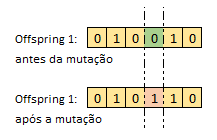
\includegraphics[scale = 0.9]{mutation.png}
\end{figure}

\subsubsection{Mutação SWAP}
A mutação swap, implementada neste trabalho, consiste basicamente na permutação de dois genes de um mesmo cromossomo. Este operador de reordenamento pode ser utilizado em problemas como o do caixeiro viajante, para prevenir a duplicação de genes, que poderia ocorrer com a mutação cartesiana.

\subsubsection{Mutação inversão}
 inversão consiste em um outro operador de reordena-mento. Neste operador, uma parte aleatória do cromossomo (situada entre dois pontos de mutação) é invertida. Esta operação é apresentada na figura \ref{fig:mutinv}

\begin{figure}[H]
\label{fig:mutinv}
  \caption{Mutação inversão}
  \centering
    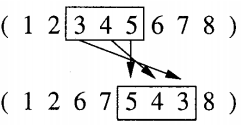
\includegraphics[scale = 0.7]{mutation_inversion.png}
\end{figure}

%------------------------------------------------

\section{Resultados}
Para a aplicação foi elaborado um formulário (\ref {fig:userview}) que possibilita ao usuário configurar os seguintes parâmetros da aplicação:
\begin{enumerate}
\item Características do algoritmo genético:
\begin{enumerate}
\item número de pontos(cidades);
\item timer;
\item tamanho da população;
\item número de gerações;
\end{enumerate}

\end{enumerate}

\begin{figure}[H]
\label{fig:userview}
  \caption{Tela de configuração do AG.}
  \centering
    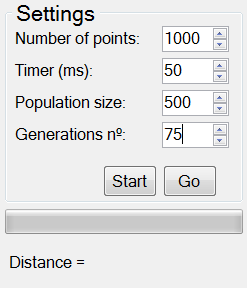
\includegraphics[scale = 0.8]{user_view.png}
\end{figure}

Ao inicializar o algoritmo genético, são realizadas as seguintes etapas:
\begin{enumerate}
\item Cria primeira população de individuos;
\item Seleciona os melhores individuos (elitismo);
\item Seleciona os indivíduos que poderão reproduzir;
\item Realiza o cruzamento entre os pais, gerando a prole;
\item Realiza a mutação dos novos individuos;
\item Atualiza a população com a nova geração de individuos, composto pelos filhos do processo de reprodução e dos melhores individuos da geração anterior.
\end{enumerate}

\begin{figure}[H]
\label{fig:tspa}
  \caption{Solução encontrada para um TSP com 15 pontos.}
  \centering
    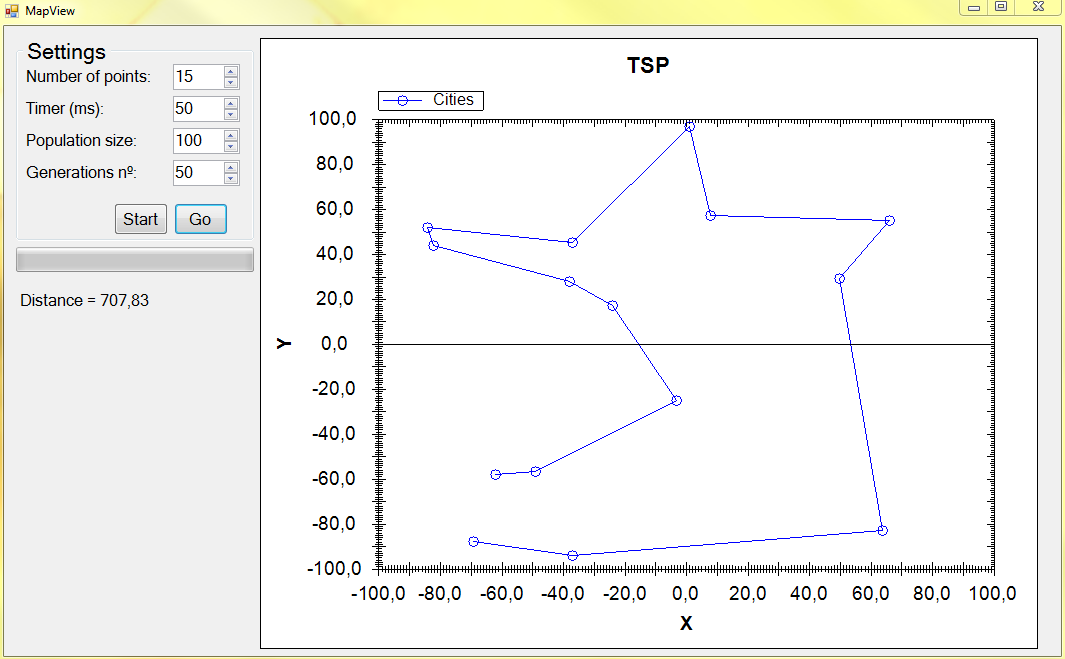
\includegraphics[scale = 0.25]{prog_tsp.png}
\end{figure}


\begin{figure}[H]
\label{fig:tspa}
  \caption{População inicial do TSP com 1000 pontos.}
  \centering
    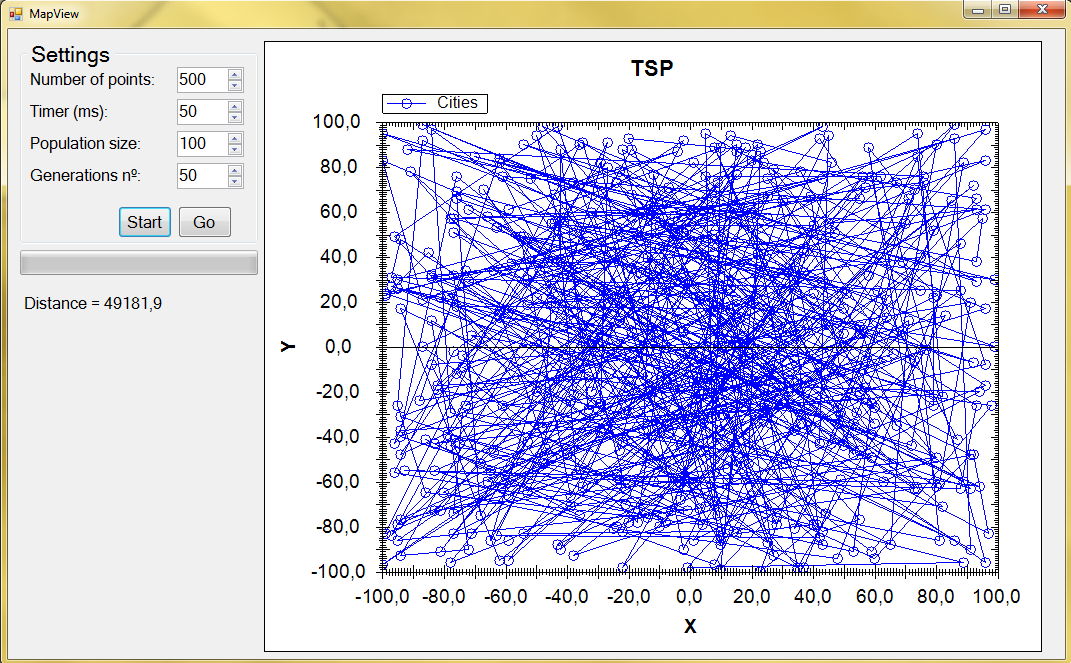
\includegraphics[scale = 0.25]{prog_tsp_a.png}
\end{figure}


%------------------------------------------------

\section{Discussão}
A medida em que o número de pontos foram aumentados (200, 500, 1000 pontos) o processamento do AG mostrou-se lento. O problema está associado à forma com que os métodos foram implementados na aplicação, de maneira a consumir um grande volume dos recursos computacionais disponíveis. Entretanto os operadores de cruzamento PMX e CX mostraram-se adequados para a resolução de problemas de ordenação, como o problema do TSP, uma vez que foi possivel encontrar soluções para problemas com um menor número de pontos. 
%----------------------------------------------------------------------------------------
%	REFERENCE LIST
%----------------------------------------------------------------------------------------

\begin{thebibliography}{99} % Bibliography - this is intentionally simple in this template

\bibitem _Linden, R. (2006).  Algoritmos Genéticos - Uma importante ferramenta da Inteligência Computacional.

\bibitem D Goldberg and R. Lingle. Alleles, loci, and the traveling salesman problem. In Proceedings of the First International Conference on Genetic Algorithms and Their Applications: July 24-26, 1985 at the Carnegie-Mellon University, Pitts-burg, PA, volume 98423, page 154. Lawrence Erlbaum, 1988.
 
\bibitem P Larranaga, C. Kuijpers, R. Murga, I. Inza, and S. Dizdare-vic. Genetic algorithms for the travelling salesman problem: A review of representations and operators. Artificial Intelli-gence Review, 13(2):129–170, 1999.

\bibitem I Oliver, D. Smith, and J. Holland. A study of permutation
crossover operators on the travelling salesman problem. In
Genetic Algorithms and Their Applications: Proceedings of
the 2nd International Conference on Genetic Algorithms. La-wrence Erlbaum Associates, Hilladale, NJ, 1987.

\end{thebibliography}

%----------------------------------------------------------------------------------------

\end{multicols}

\end{document}